\documentclass{beamer}
\usetheme{Madrid}
\usepackage[utf8]{inputenc}
\usepackage[english]{babel}
\usepackage{subcaption}

% Tikz
\usepackage{tikz}
% \usetikzlibrary{decorations.fractals}
% \usetikzlibrary{lindenmayersystems}

\newcommand{\R}{\ensuremath{\mathbb{R}}}
\newcommand{\N}{\ensuremath{\mathbb{N}}}
\newcommand{\B}{\ensuremath{\mathcal{B}}}

\title{Hausdorff Measure}
\author{Jack Maloney}

\begin{document}

\begin{frame}
    \titlepage
\end{frame}

\begin{frame}{Motivation}
    \begin{figure}[h]
    	\begin{subfigure}{.3\textwidth}
    	  	\centering
    		\begin{tikzpicture}
    			\draw (0,0) -- ++(-1,1/2) -- cycle;
    		\end{tikzpicture}
    		\caption{A Line}
    	\end{subfigure}
    	\begin{subfigure}{.3\textwidth}
    		\centering
    		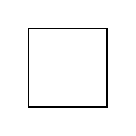
\begin{tikzpicture}
    			\draw (0,0,0) -- ++(-1,0,0) -- ++(0,-1,0) -- ++(1,0,0) -- cycle;
    		\end{tikzpicture}
    		\caption{A Square}
    	\end{subfigure}
    	\begin{subfigure}{.3\textwidth}
    		\centering
    		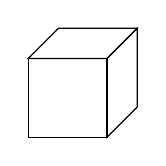
\begin{tikzpicture}
    			\draw (0,0,0) -- ++(-1,0,0) -- ++(0,-1,0) -- ++(1,0,0) -- cycle;
    			\draw (0,0,0) -- ++(0,0,-1) -- ++(0,-1,0) -- ++(0,0,1) -- cycle;
    			\draw (0,0,0) -- ++(-1,0,0) -- ++(0,0,-1) -- ++(1,0,0) -- cycle;
    		\end{tikzpicture}
    		\caption{A Cube}
    	\end{subfigure}
    	\caption{Three Subsets of \(\R^3\)}
    \end{figure}
\end{frame}

\end{document}
